\chapter{Estructuras de micro-escala en la crom\'osfera solar}

La atm\'osfera solar se divide en las siguientes capas: la fot\'osfera, crom\'osfera, regi\'on de transici\'on y la corona solar. Cada una de estas regiones poseen distintos reg\'imenes de densidad y temperatura ilustr\'andose en la figura \ref{atmosfera_solar}.

\begin{figure}[h]
\centering
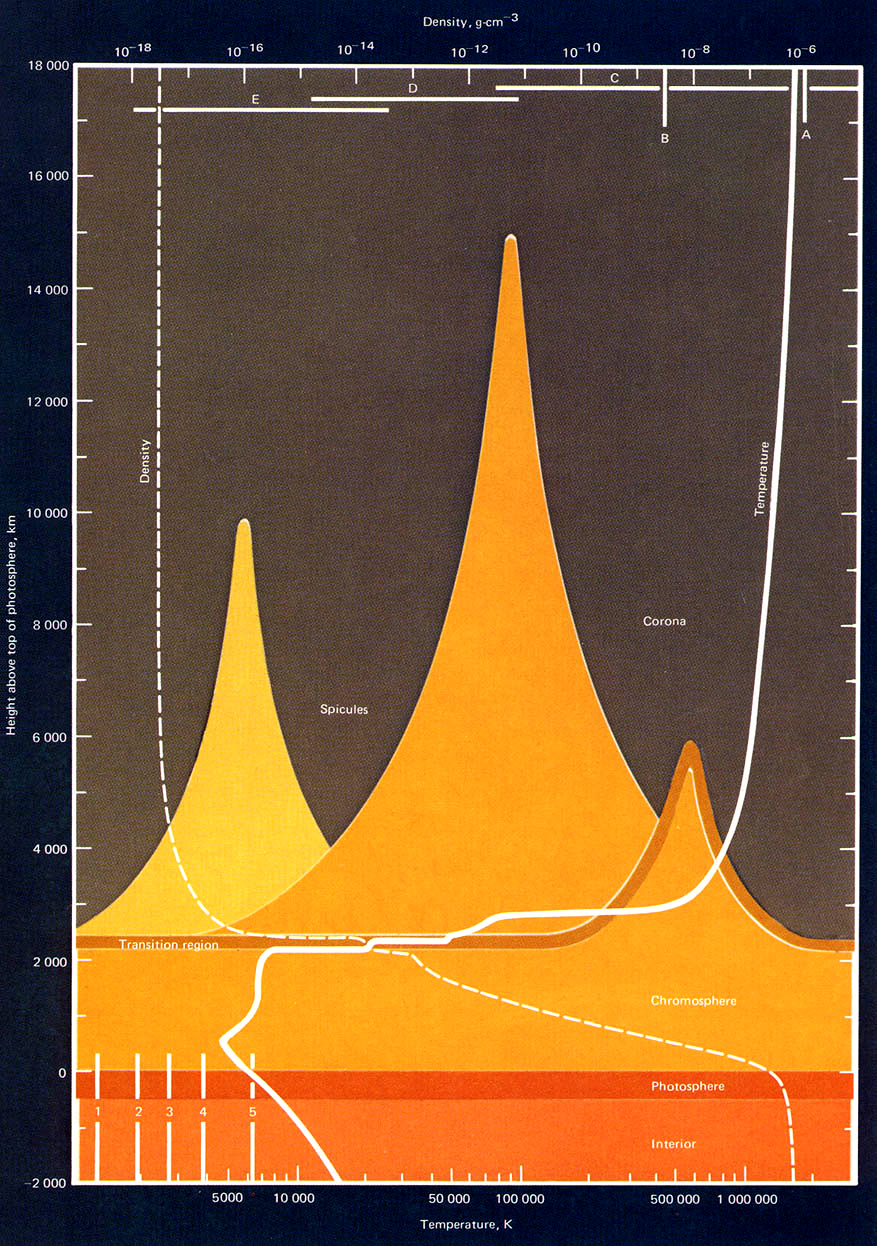
\includegraphics[scale=.65]{atmosfera_1}
\caption{Ilustraci\'on de la estructura de la atm\'osfera del Sol (tomada de https://history.nasa.gov/SP-402/p2.htm). \newline
*Existe debate sobre si la regi\'on de transici\'on es una regi\'on por s\'i misma o forma parte de la Crom\'osfera. Independientemente de esto, se localizar\'ia entre la Crom\'osfera y la Corona Solar.} \label{atmosfera_solar}
\end{figure}

La atm\'osfera solar est\'a descrita por la f\'isica de un plasma magnetizado. El estado del plasma y/o su interacci\'on con el campo magn\'etico establecen mecanismos de emisi\'on en pr\'acticamente todo el espectro electromagn\'etico. Estos mecanismos consisten en trancisiones at\'omicas (que pueden ser ionizantes, de recombinaci\'on y tipo ligado-ligado) y mecanismos de emisi\'on libre-libre como radiaci\'on \emph{bremsstrahlung}, radiaci\'on sincrotr\'onica y radiaci\'on plasma.  *agregar referencia*

La atm\'osfera solar se extiende desde los niveles fotos\'ericos hasta el medio coronal pasando por el medio cromosf\'erico, involucrando una escala de longitud de $1R_{\odot}$--$3R_{\odot}$ *agregar referencia*. La \emph{fot\'osfera} se constituye de gr\'anulos convectivos de peque\~na escala ($10^3$~km), separados de entre s\'i por capas intergranulares, las cuales concentran elementos de alto flujo magn\'etico ($|B| \le 1\mbox{kG}$). La escala temporal de la ocurrencia de un gr\'anulo es de unos minutos aproximadamente. La \emph{crom\'osfera} (ver fig. \ref{atmosfera_solar}) es una capa que se extiende por alrededor de $2\times 10^3$~km. Emite intensamente en la l\'inea H$\alpha$ ($\lambda=6563~\mbox{\AA}$) y ultravioleta. Similarmente a la fot\'osfera, la base de la crom\'osfera presenta gr\'anulos con una escala de tama\~no relativamente mayor concentrando flujo magn\'etico, el cual est\'a asociado en unos casos con flujos verticales de plasma llamados \emph{esp\'iculas} o a microarcos magn\'eticos en otros casos~\citep{NASAweb}. M\'as all\'a de la base de la crom\'osfera cambia la condici\'on en la presi\'on dominante, ya que mientras la presi\'on del gas domina a niveles fotosf\'ericos, a estos niveles esta condici\'on se invierte y las distribuciones de brillo observadas est\'an dominadas por la geometr\'ia del campo magn\'etico. *agregar referencia*

%Por su parte, la \emph{corona} es una de las partes de la atm\'osfera m\'as desconocidas para la ciencia hasta el momento. Su mayor misterio es que conforme la densidad decrementa, la temperatura en lugar de decrementar tambi\'en se incrementa. Este fen\'omeno se presenta a\'un m\'as radicalmente en una capa que antecede a la Corona conocida como la regi\'on de transici\'on (TR por su nombre en ingl\'es "Transition Region"). Particularmente, en dicha regi\'on a\'un no est\'a claramente explicado el cambio radical que pasa de $10^4$K a $10^5$ K en una distancia de $1000$~km (v\'ease fig.~\ref{atmosfera_solar}).

El rango de temperaturas implicado en este cambio de morfolog\'ia, de gr\'anulos a estructuras filamentarias magn\'eticas (\emph{en ingl\'es loops}) es de $2\times 10^5~\mbox{K} < T < 10^6~\mbox{K}$

El escenario anterior propone que, a trav\'es de las ep\'iculas se establece un mecanismo continuo de transferencia de material y energ\'ia hacia la corona solar, por lo que se han propuesto modelos que expliquen tanto la din\'amica y estructura t\'ermica de una condici\'on conocida como \emph{Sol Quieto}, en referencia a regiones del Sol que excentas de cualquier manifestaci\'on de actividad observable *agregar referencia*. Modelos est\'aticos de atm\'osferas referentes, son los desarrollados por Vernazza et al. 1991 (VAL), Fontenla et al. 1993 y Avrett y Loeser 2008 (C7). En ellos, se ajusta una atm\'osfera hidrost\'atica, promediando propiedades estratificadas en una aproximaci\'on plano-paralela hasta reproducir el correspondiente espectro emergente para un conjunto de observaciones seleccionadas. A\'un cuando la f\'isica de aquellos modelos es bastante realista, no toma en cuenta la din\'amica a escala angular menor al poder de resoluci\'on angular de las observaciones actuales.

Con el advenimiento de instrumentos que observan en el rango UV, como el Interface Region Imaging Spectrograph (IRIS) y el Solar Dynamics Observatory (SDO), muestra que la estructura de la atm\'osfera (y muy particularmente, de la crom\'osfera) es tan complejamente distribuida, que un modelo que promedie propiedades como en el p\'arrafo anterior no puede capturar el escenario real. *agregar referencia*

En a\~nadidura, las  observaciones del experimento VAULT (Very high Angular resolution ULtraviolet Telescope por sus siglas en ingl\'es) complementan la evidencia de una estructura cromosf\'erica y de la existencia de peque\~nos loops frios \citep{VAULT1}, los cu\'ales confirman la presencia de campos magn\'eticos.
VAULT es un proyecto de exploraci\'on espacial que data de 1999 y que busca estudiar la conexi\'on entre la corona y la crom\'osfera solar al observar la l\'inea espectral m\'as fuerte del sol, la Ly$\alpha$ a 1216A.
La resoluci\'on angular de sub-arcosegundos ($\approx$.3") permite ver directamente los peque\~nos loops f\'ios en la estructura de Sol Quieto. El parecido de los resultados entre los modelos y las observaciones indican que la explicaci\'on de las estructuras finas observadas en t\'erminos de loops frios es plausible.

Como se muestra en la figura \ref{fig:vault_compare} las im\'agenes de VAULT nos permiten mejorar la calidad de nuestras observaciones, permiti\'endonos tener un mejor entendimiento de la composici\'on de la atm\'osfera solar (n\'otese tambi\'en la calidad de la figura Y). *agregar referencia*

\begin{figure}[ht]
\centering
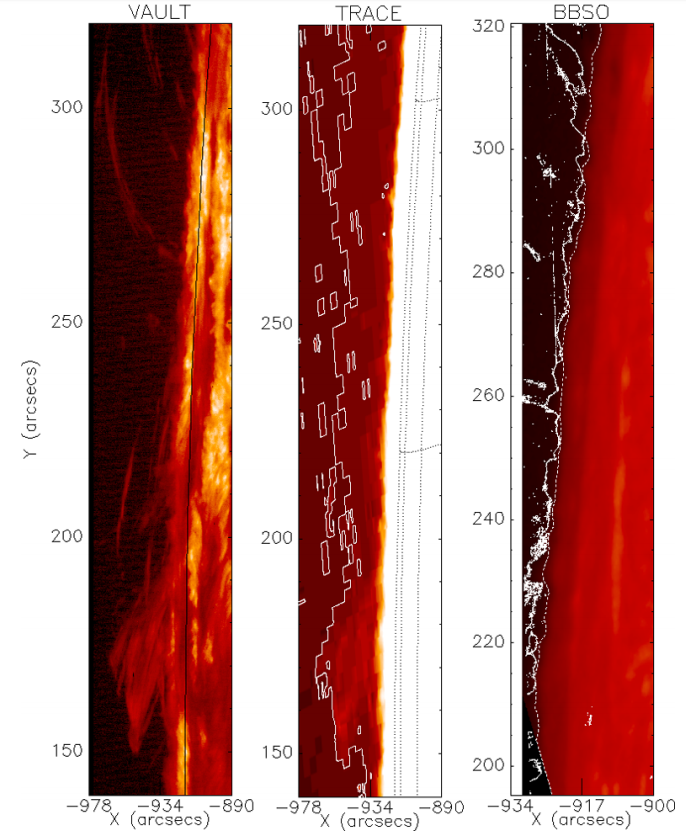
\includegraphics[scale=0.6]{vault_comparison}
\caption{"Fuente: Vourlidas, et al., 2009"}
\label{fig:vault_compare}
\end{figure}

\begin{figure}[ht]
\centering
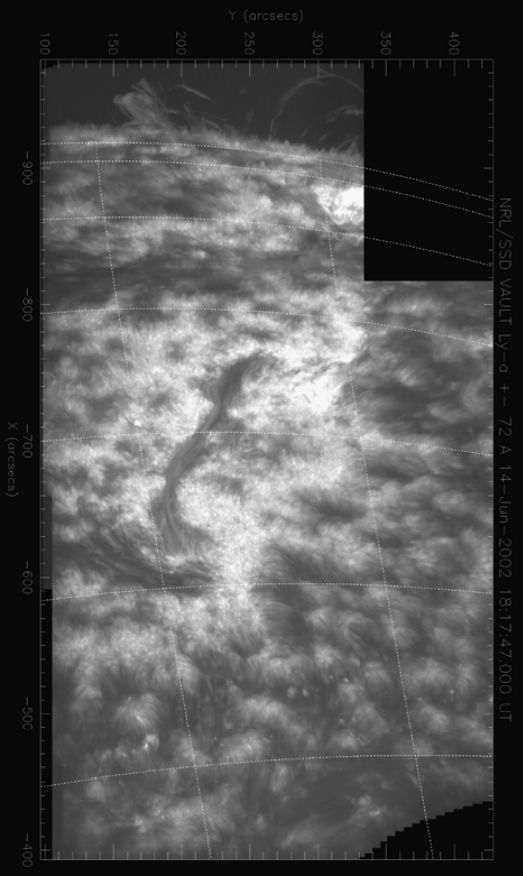
\includegraphics[scale=0.6]{vault_complete}
\caption{"Fuente: Vourlidas, et al., 2009}
\label{fig:vault_complete}
\end{figure}

Actualmente se esta develando la estructura en el disco solar en ondas mm ($\lambda=3$~mm) con una resoluci\'on 3.7'' $\times$ 2.5''.*agregar referencia* La distribuci\'on de brillo es muy similar a la observada en su contraparte ultravioleta por el sat\'elite IRIS (ver Figura ~\ref{fig:chromosphericnet1}): una red cromosf\'erica constitu\'ida de gr\'anulos con temperatura de brillo $T_{\tiny{\mbox{b}}}=6500$~K en promedio (\cite{2018A&A...619L...6N}*agregar referencia*). Lo anterior sugiere que la radioemisi\'on en ondas mm esta  ubicada en la regi\'on cromosf\'erica dispuesta en flujos emergentes o estructuras filamentarias observadas al limbo (loops) (ver Figura ~\ref{fig:chromosphericnet2})

Carlsson y Sten (1994) modelan bidimensionalmente la emisi\'on emergente t\'ermica libre-libre cromosf\'erica a longitudes de onda milim\'etricas y submilim\'etricas. La temperatura de brillo resultante var\'ia sensiblemente en el tiempo debido a la propagaci\'on de ondas de choque y modos de oscilaci\'on, contabilizando una complejidad m\'as realista para la temperatura local del gas en las capas de formaci\'on del continuo de emisi\'on. Las escalas angulares involucradas en estos resultados est\'an por debajo de los 0.1''. Asi, la emisi\'on milim\'etrica y submilim\'etrica dependen fuertemente. Loukitcheva et al. 2004 refieren que las el escenario din\'amico de la estructura cromosf\'erica es consistente con la emisi\'on milim\'etrica y submilim\'etrica observada---\textbf{revisa la redacci\'on de la ulitma parte de este p\'arrafo}


Se puede decir entonces que el conocimiento con respecto al impacto de las micro estructuras magn\'eticas en la emisi\'on milim\'etrica y submilim\'etrica es escaso. Sin embargo existen esfuerzos recientes por comprender este impacto. Por ejemplo, \emph{PakalMPI} (De la Luz 2010) es un c\'odigo que resuelve la ecuaci\'on de transferencia radiativa en tres dimensiones en una aproximaci\'on plano-paralela, cuya estratificaci\'on sigue perfiles conocidos de densidad y temperatura y bas\'andose de los modelos semi-emp\'iricos VAL y C7, lo cuales, bajo determinadas modificaciones se introducen en c\'odigo \emph{PakalMPI}.

\begin{figure}[ht]
\centering
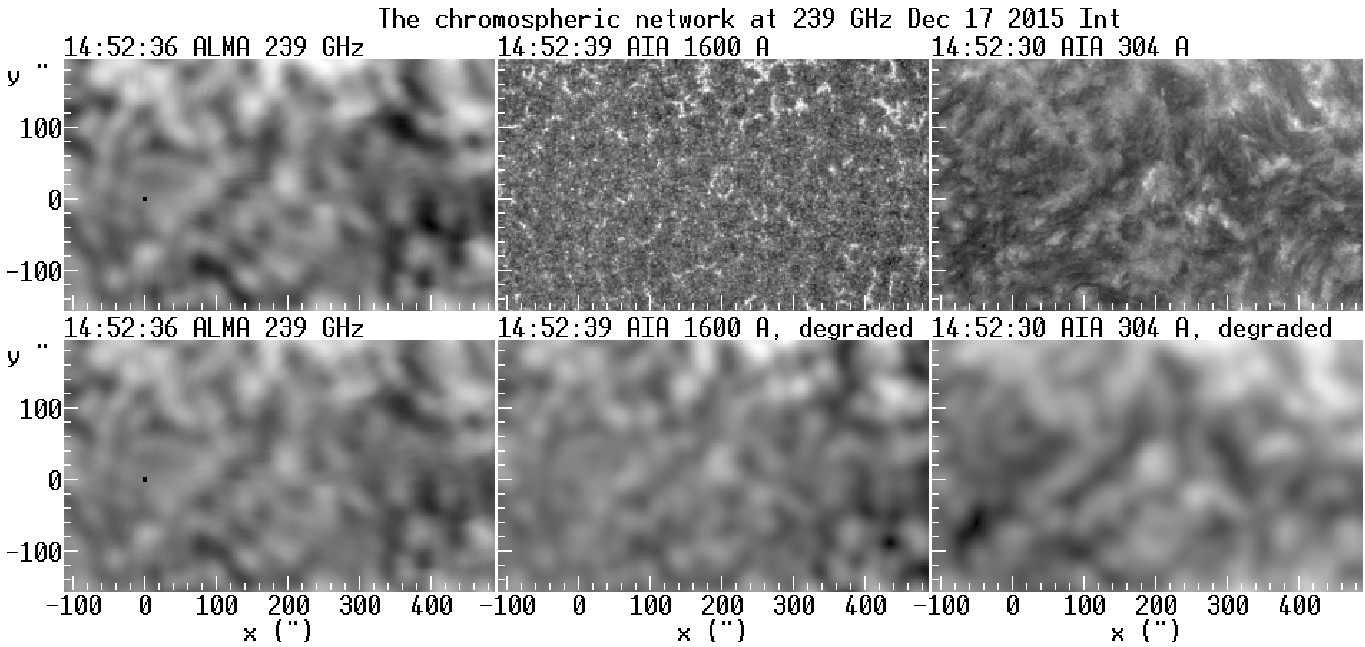
\includegraphics[scale=0.4]{ALMA}
\caption{Im\'agenes de la red cromosf\'erica en las cercan\'ias del centro del disco solar durante el 17 de Diciembre de 2015 a 239~GHz (1.2~mm) junto con im\'agenes de AIA-SDO a 1400~$\mbox{\AA}$ (continuo) y 304~$\mbox{\AA}$ (emisi\'on de HeII). En el rengl\'on de abajo se muestran las im\'genes de AIA-SDO degradadas a las resoluci\'on de ALMA~\cite{2017A&A...605A..78A}.}
\label{fig:chromosphericnet1}
\end{figure}

\begin{figure}[ht]
\centering
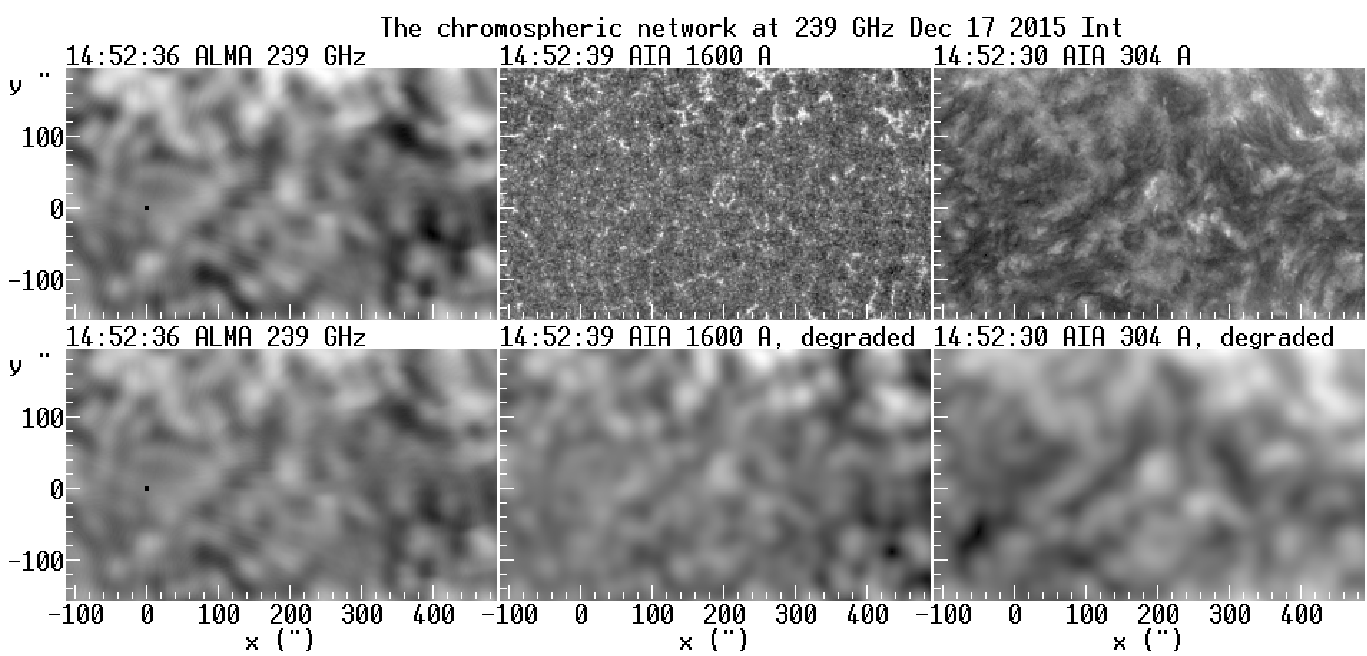
\includegraphics[scale=0.4]{ALMA_I}
\caption{Im\'agenes de ALMA mostrando el disco completo durante el 17 de Diciembre de 2015 comparadas con im\'agenes en otras longitudes de onda. \emph{Arriba de izquierda a derecha: }im\'agen de ALMA a 239~GHz; la misma pero degradada a la resoluci\'on de la im\'agen de 100~GHz; e ima\'agen de ALMA a 100~GHz sin degradar. \emph{Rengl\'on inferior: } H$\alpha$ de la red GONG; im\'agen a 1600~$\mbox{\AA}$ de AIA-SDO; y magnetograma de HMI-SDO~\cite{2017A&A...605A..78A}.}
\label{fig:chromosphericnet2}
\end{figure}

%\begin{figure}[ht]
%\centering
%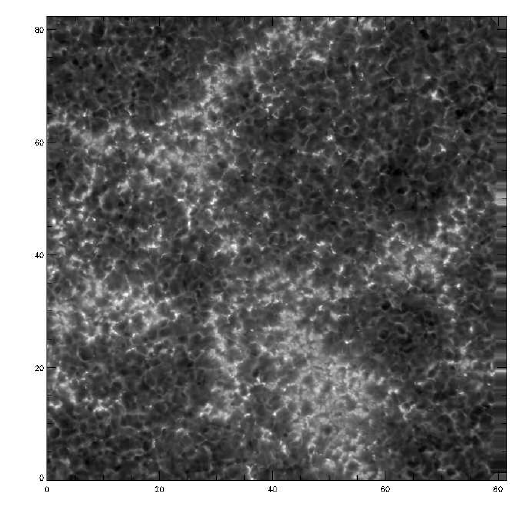
\includegraphics[scale=0.5]{chromospheric_network2}
%\caption{ Red cromosf\'erica solar observada desde el Telescopio Solar Sueco (Swedish Solar Telescope) en la l\'inea H Ca II.
%\newline Fuente: https://www.researchgate.net/figure/The-chromospheric-network-as-observed-with-the-Swedish-Solar-Telescope-in-the-Ca-II\_fig8\_259104617}
%\label{chromospheric_network2}
%\end{figure}



%En la figura \ref{fig:chromosphericnet} se observa una imagen tomada en la l\'inea de c\'alcio de la red cromosf\'erica, mientras que en la figura 

\section{El c\'odigo \emph{Pakal}}
%Descripci\'on del c\'odigo, puntualmente hay qu\'e explicar primero para qu\'e sirve actualmente y a partir de ello, plantear las modificaciones.
Como se mencion\'o anteriormente, esta tesis busca extender el c\'odigo Pakal 2011\citep{Pakal}. Dicho programa es un modelo num\'erico inovador que pretende resolver la ecuaci\'on de transferencia radiativa en una geometr\'ia tridimensional (3D), usando una aproximaci\'on para una atm\'osfera localmente plano paralelo; lo anterior utilizando un sistema inteligente. Con este programa se generan las capas estratificadas de la atm\'osfera en una estructura l\'ogica. La salida del c\'odigo puede ser en forma de mapas bi-dimensionales o un perfil de una dimensi\'on, que reproduce las observaciones con alta presici\'on, dando informaci\'on f\'isica detallada acerca del entorno donde la radiaci\'on fue generada y/o transmitida.

Pakal se encuentra dividido en cuatro distintos m\'odulos: El modelo num\'erico, la geometr\'ia, los m\'etodos num\'ericos y las funciones f\'isicas. Estos cuatro m\'odulos pueden ser modificados independientemente sin afectar el funcionamiento de los otros. En esta tesis se modifica el m\'odulo de las funciones f\'isicas donde se resuelve la ecuaci\'on de transferencia.

Como todo modelo, Pakal est\'a basado en una serie de supuestos que le brindan una serie de fortalezas, pero tambi\'en una serie de limitantes; las cuales se presentar\'an a continuaci\'on. Con relaci\'on a sus supuestos, Pakal presenta un modelo aplicado a una geometr\'ia solar radial 3D, asumiendo una atm\'osfera local plano-paralela, y una emisi\'on t\'ermica de radio libre-libre de gas hidr\'ogeno-helio en equilibrio termodin\'amico. Para sus c\'alculos Pakal asume un grosor de la Crom\'osfera de 2200km. Adem\'as tambi\'en utiliza perfiles radiativos precalculados de densidad y temperatura (basado en modelos hidrost\'aticos, hidrodin\'amicos o MHD) para calcular la emisi\'on de una fuente de estructuras 3D con alta resoluci\'on espacial. En todo momento Pakal asume un estado de Sol Quieto y la ausencia de campos magn\'eticos. El t\'ermino Sol Quieto hace referencia a regiones del Sol que se encuentran excentas de cualquier manifestaci\'on de actividad observable. Pakal resuelve la ecuaci\'on de transferencia radiativa en un conjunto de l\'ineas dirigidas de la fuente al observador.

En relaci\'on con las limitaciones de Pakal, si bien este permite la entrada de observaciones, no est\'a basado en ellas, y por lo tanto los resultados no representan por completo las caracter\'isticas f\'isicas existentes. De igual forma, Pakal se encuentra limitado a la crom\'osfera. Adem\'as Pakal omite la emisi\'on \emph{gyrosynchrotron} al despreciar los campos magn\'eticos. Finalmente, el c\'odigo de Pakal no logra reproducir en un 100\% las funci\'ones de densidad y temperatura del plasma solar.
 
Pakal ha demostrado poder mejorar el tiempo de integraci\'on hasta por un orden de magnitud comparado a c\'odigos de integraci\'on lineal. Por ejemplo, en una prueba que utilizaba 32 procesadores de una m\'aquina Cray del CNS en san Luis Potos\'i, se generaron espectros sint\'eticos de 32 frecuencias, con pasos de integraci\'on de 1km del centro del disco solar en aproximadamente 3 segundos. Adem\'as, Pakal puede correr en clusters, supercomputadoras y computadoras personales. Los resultados de Pakal han sido probados por su robustez. Particularmente, se realizaron satisfactoriamente pruebas de convergencia y estabilidad de la parte num\'erica y del sistema experto, las cu\'ales son presentadas en De la Luz et al. (2010). Por \'ultimo, Pakal permite modelar computacionalmente modelos semi emp\'iricos. 

En esta tesis se propone una extensi\'on en el m\'odulo de funciones f\'isicas (denominado Jaguar). Particularmente se agrega el efecto de los campos magn\'eticos a la ecuaci\'on de transferencia al agregar la componente de la presi\'on magn\'etica. Lo anterior convierte al modelo hidrodin\'amico que se usa actualmente en un modelo magnetohidrost\'atico. Con esta adici\'on (1) se puede generar un escenario m\'as apegado a las observaciones f\'isicas de la atm\'osfera solar, y (2) se facilita la adaptaci\'on del c\'odigo ante la adici\'on de cualquier modelo de campo magn\'etico.



\section{Sobre el Sol quieto y la emisi\'on submilim\'etrica solar}

Hist\'oricamente el concepto de Sol quieto se ha visto modificado, por lo que antes que todo se recomienda al lector tener precauci\'on en asumir una consistencia conceptual en textos de diferentes tiempos. Hoy en d\'ia, este t\'ermino se refiere a dos conceptos. Primeramente se puede referir a las regiones del Sol que abarcan todas las regiones de campo magn\'etico cerrado (excluyendo las regiones activas), claramente demarcando el territorio de Sol quieto de los hoyos coronales, que abarca regiones de campo magn\'etico abierto.
Segundamente, se refiere a un estado solar general que ocurre cada 11 a\~nos y se caracteriza por una actividad solar baja. Esta actividad solar baja b\'asicamente es equivalente a la primera definici\'on antes mencionada. En esta tesis cuando se utiliza el concepto de sol quieto, nos estamos refiriendo a la primer definici\'on, la cual describe el fen\'omeno solar de inter\'es. Se asume \'unicamente el estado de sol quieto debido a la complejidad del Sol activo. Sin embargo, el entendimiento del sol quieto tambi\'en nos ayudar\'ia a entender mejor el Sol Activo. Concretamente, la correcta caracterizaci\'on del Sol Quieto nos permitir\'ia entender el fondo de radiaci\'on del Sol Activo.

Una caracter\'istica relevante del Sol quieto para esta tesis es el de la intensidad de sus campos magn\'eticos. Particularmente los campos magn\'eticos en Sol quieto, medidos seg\'un las l\'ineas espectrales de Zeeman, contienen un campo de B== .1 - .5G, mientras que sus fuerzas absolutas de campo en elementos resueltos var\'ian entre B = 10-50G *agregar referencia*. Estos valores se utilizan en el modelo computacional propuesto en este texto.

Si bien se conocen los rangos de la magnitudes de los campos magn\'eticos del Sol quieto *agregar referencia*, existe una dificultad en medir las magnitudes concretas de estos debido a corrientes desconocidas y condiciones no libres de fuerza. Lo anterior ocasiona que se tengan que calcular extrapolaciones a lo largo de la crom\'osfera y la regi\'on de transici\'on para obtener valores aproximados. 

La región de transisión es una capa muy delgada e irregular de la atmósfera solar que separa la corona caliente de una cromósfera mucho más fría. El calor fluye de la corona a la cromósfera en un proceso que produce esta pequeña regi\'on donde la temperatura cambia rápidamente de 1,000,000C hasta 20,000C. A esas temperaturas, el hidrógeno es ionizado, provocando que la luz emitida en esta región sea dominada por iones como C IV, O IV y Si IV (carbono, oxígeno y silicón); emitiendo luz en la región ultravioleta del espectro solar *agregar referencia*, es la de la nasa NASA 2014.
%(solarscience.msfc.nasa.gov/t_region.shtml)

Otra caracter\'istica importante del Sol quieto para esta tesis es la emisi\'on milim\'etrica del plasma. Se ha comprobado que la observaci\'on de la emisi\'on milim\'etrica del plasma en Sol Quieto es equivalente a observar la totalidad de las emisiones de la Crom\'osfera Solar cuando est\'a en el estado solar de Sol Quieto \citep{millimeter}. Con la emisi\'on milim\'etrica se puede aproximar el grado de ionizaci\'on de la atm\'osfera solar; y se pueden inferir aproximaciones de la temperatura, la densidad y la presi\'on que hay en ella. Estas \'ultimas aproximaciones se realizan seg\'un diferentes modelos; los cuales se pueden conceptualizar como emp\'iricos, semi-emp\'iricos y observacionales. 
*Enrique*
******
La emisión de radio del Sol Quieto es la suma de la emisión cromosférica opticamente gruesa y corona ópticamente delgada superpuesta. Para longitudes de onda debajo de algunos cm (frecuencias sobre varios cientos de Mhz) la contribución coronal en la emisión se vuelve negligible y una de las medidas de temperatura de la cromósfera en la profundidad óptica a esa longitud de onda concreta. Por lo que teniendo observaciones milimétricas multifrecuencia de la temperatura de brillo del sol quieto uno puede obtener la temperatura y de medida de emisión de la cromósfera.
*********


Independientemente del tipo de modelo, por definici\'on, todos tienen limitaciones en sus c\'alculos de temperatura, densidad y presi\'on. En el modelo propuesto, se busca robustecer el modelo Pakal mediante la anexi\'on de el efecto te\'orico de los campos magn\'eticos. Esta anexi\'on se puede justificar, por diferentes teor\'ias y observaciones. Por ejemplo, un estudio reciente por Meunier (2018) propone que las peque\~nas regiones de campo magn\'etico contribuyen a la emisi\'on cromosf\'erica y por consiguiente a la emisi\'on milim\'etrica. Lo anterior, como se explic\'o previamente, afectar\'ia a los c\'alculos de la temperatura, la densidad y la presi\'on de la crom\'osfera; haci\'endolos te\'oricamente m\'as precisos.
